\begin{newpage}
	
	\section{Grundlagen}
	\label{sec:Grundlagen}

  \subsection{Begriffe}
  \label{sub:begriffe}
    Nachfolgend sollen die wichtigsten Begriffe definiert werden, um ein Einheitliches Verständnis zu garantieren.

    \subsubsection{Vehicle}
    \label{ssub:vehicle}
      Ein Vehicle $V$ beschreibt in dieser Arbeit ein Fahrzeug, welches im Dienste der öffentlichen Verkehrsbeförderung steht. Beispielsweise Bus, U- \& S-Bahn, Interrail Züge aber auch Zahnradbahn oder gar Funicular-Services\footnote{\url{https://en.wikipedia.org/wiki/Funicular}}. Das private Automobil fällt folglich nicht unter diese Definition.
    % subsubsection vehicle (end)

    \subsubsection{Station}
    \label{ssub:station}
      Eine Station $S$ ist eine Haltestelle, die von einem Vehicle $V$ während eines Trips $T$ angefahren wird. Die Station definiert dabei die Ankunfts- und Abfahrtszeiten, wann ein Vehicle an dieser Station haltet und wann es diese zur weiterfahrt wieder verlässt. Ankunfts- und Abfahrtszeit seien wie folgt definiert:\\

      arrival time $ := t_{ari}$\\
      departure time $ := t_{dep}$

    % subsubsection station (end)

    \subsubsection{Polyline}
    \label{ssub:polyline}
      Eine Polyline $P$ ist eine Kurve die sich durch eine Sequenz an Punkten $p_1, \dotsc, p_n$ definiert.

    % subsubsection polyline (end)

    \subsubsection{Trip}
    \label{ssub:trip}
      In dieser Arbeit wird immer wieder der Begriff "`Trip"' Verwendung finden. Ein Trip $T$ sei mit folgenden Eigenschaften definiert:
      \begin{itemize}
        \item $T = \{s_1, \dotsc, s_n \;|\; s \in S, n \in \mathbb{N}, n \geq 2 \}$

        \item Ein Trip $T$ wird dabei von genau einem Vehicle $V$ bedient. Daraus folgt $T$ mit dem Mapping: $T \mapsto V$ ist Injektiv\footnote{Ein Trip wird von genau einem Vehicle ausgeführt} zu $V$. 

        \item Die Bewältigung der Strecke $\{A,B \;|\; A, B \in S\}$ gilt als ein einziger Trip. Ein Trip beginnt also genau dann, wenn die momentane Zeit $t_{cur}$ mit der Abfahrtszeit $t_{dep}$ übereinstimmen $\Rightarrow t_{cur} = t_{dep} $ .

        \item Der Rückweg $\{B, A \ni T \;|\; A, B \in S\}$ ist nicht in einem Trip $T$ enthalten, sondern würde als ein neuer Trip erfasst werden.
      \end{itemize}
      
    % subsubsection trip (end)

    \subsubsection{Route}
    \label{ssub:route}
      Eine Route $R$ besteht aus einer Anzahl an Trips $T$.
      \begin{itemize}
        \item $R = \{ t_1, \dotsc, t_n \;|\; t \in T, n \in \mathbb{N}, n \geq 1 \}$

        \item $R$ mit dem Mapping: $R \mapsto T$ ist Surjektiv\footnote{Eine Route kann mehrere Trips besitzen, wohingegen ein Trip nur zu einer Route zugehörig sein kann} 
      \end{itemize}
    % subsubsection route (end)

  % subsection begriffe (end)

	\subsection{GTFS Datenformat}
	\label{ssec:gtfs_datenformat}
		Das GTFS (General Transit Feed Specification) ist eine Datenstandardisierung die von Google im Jahr 2006 entwickelt wurde. Vor dessen Einführung gab es weder eine einheitliche Standardisierung, noch ein "`de facto Standard"' für die Fahrpläne des Öffentlichen Nahverkehrs in den USA. GTFS ermöglichte es Transit Organisationen ihre Daten für dritte zu öffnen und ist heute das weit verbreitetste offene Datenformat für den öffentlichen Nahverkehr.\parencite[S. 2]{roush}\\

    Ein GTFS Feed besteht aus mindestens 6 und maximal 13 \texttt{csv-Dateien}, die im \texttt{.txt} Format vorliegen müssen. Die Struktur eines Feeds lässt sich in Worten wie folgt beschreiben:

    \begin{quote}
      \textit{Ein GTFS Feed besteht aus einer oder mehreren Routen. Jede Route (\texttt{routes.txt}) hat einen oder mehrere Trips (\texttt{trips.txt}). Jeder Trip besucht eine Abfolge von Stops (\texttt{stops.txt}) zu einer bestimmten Zeit (\texttt{stop\_times.txt}). Trips und Stop-Zeit beinhalten nur die Tageszeit Informationen. Der Kalender (calendar.txt und \texttt{calendar\_dates.txt}) bestimmt dann, an welchen Tagen ein bestimmter Trip stattfindet.} \cite[S. 8]{zervaas}
    \end{quote}

		Vor allem für digitale Produkte, wie zum Beispiel Trip-Planer, die viele verschiedene Fahrpläne von unterschiedlichen Unternehmen in ihren Service integrieren müssen, ist ein standardisiertes Datenformat unbedingt notwendig. 
		Ansonsten müsste jede App die Entwickelt wird, auf das Datenformat der jeweiligen Verkehrsunternehmen angepasst werden. Das wiederum bedeutet, dass je nach Implementierung innerhalb dieser Unternehmen, die Datenformate gänzlich voneinander abweichen können. Für jeden dieser Anbieter müsste folglich eine ganz eigene Datenverarbeitungslogik geschrieben werden.
    Darüber hinaus könnte natürlich jedes Verkehrsunternehmen jederzeit sein eigenes Datenformat ändern, was zur Folge hat, dass ein App-Entwickler diese Änderungen auch in sein Produkt übernehmen muss. Bei einer Integration von Daten, aus beliebig vielen unterschiedlichen Verkehrsunternehmen (Beispiel: Trip-Planer für ein ganzes Land), könnten sich laufend Änderungen ergeben die integriert werden müssen, oder das eigene Produkt würde nicht mehr zuverlässig funktionieren. Dies übersteigt die Wartbarkeit und Robustheit einer App, denn sie würde möglicherweise immer dann nicht mehr funktionieren, wenn ein Dritter entscheidet sein eigenes Datenformat zu ändern. Aus diesem Grund gab es bis vor einiger Zeit nahezu keine Trip oder Routen-Planer Anwendungen die nicht von den Verkehrsunternehmen selbst stammten würden. Der Status Quo war: Jedes Verkehrsunternehmen hat seine eigene Anwendung für die Fahrplanauskunft. Unter anderem aus diesem Grund erfolge die Adaption an das neue GTFS Format sehr schnell und so sind heute die meisten öffentlich verfügbaren Fahrpläne im GTFS Format auf Plattformen wie: \url{http://transitfeeds.com} oder \url{https://transit.land/} frei verfügbar.\footnote{Momentan besitzt Transitfeeds 535 Feeds (Stand 18.08.2017)}\\

    Trotz der Standardisierung durch GTFS gibt es immer noch diverse Freiräume in der Umsetzung des Formats. Wie anfangs erwähnt wurde, beträgt die Anzahl der Dateien die für ein gültiges GTFS Feed benötigt werden nur Sechs. Es sind allerdings bis zu 13 Dateien möglich. Dies zeigt wie viele unterschiedliche Informationen ein GTFS Feed bereitstellen kann, aber nicht muss. 
    Auch innerhalb der Dateien gibt es Felder die vorhanden sein "`müssen"' oder nur "`dürfen"'. Beispielsweise muss das Feld \texttt{route\_short\_name} in \texttt{routes.txt} vorhanden sein, aber \texttt{route\_desc} (Route Description) nicht. Der Interpretationsspielraum lässt sich aber noch weiter veranschaulichen, wenn wir uns Tabelle ~\ref{table:gtfs_differences} ansehen. In dieser Tabelle sind Zwei Einträge aus unterschiedlichen GTFS Feeds aufgelistet.
    Wir sehen, dass die Spalte \texttt{route\_id} bei Stuttgart-VVS als Zahlenwert angegeben wird, wohingegen Boston-MBTA einen Text verwendet.

    \begin{longtable}{|>{\raggedright \arraybackslash}p{3.0cm}|>{\raggedright \arraybackslash}p{2.0cm}|>{\raggedright \arraybackslash}p{3.5cm}|>{\raggedright \arraybackslash}p{5.5cm}|}
    \caption{Unterschiede innerhalb GTFS} 
    \label{table:gtfs_differences}\\
      \hline
       & route\_id & route\_short\_name & route\_long\_name\\
      \hline
      Stuttgart-VVS & 379 & U1 & Fellbach - Hauptbahnhof - Vaihingen\\
      \hline
      Boston-MBTA & Blue Line & Blue & Bowdoin - Wonderland\\
      \hline
    \end{longtable}

    "`Blue Line"' ist dabei die Bezeichnung der U-Bahnlinie\parencite{wiki_blue_line}. Wir sehen also, dass Stuttgart-VVS die \texttt{route\_id} zur eindeutigen Identifizierung mittels Zahlenwert verwendet wohingegen Boston-MBTA dieses Feld nutzt, um den Namen der Linie zu beschreiben. Angenommen wir verwenden die \texttt{route\_id} in einer Benutzeroberfläche wie in Abbildung~\ref{fig:gtfs_differences}.

    \begin{figure}[htbp]
      \begin{center}
        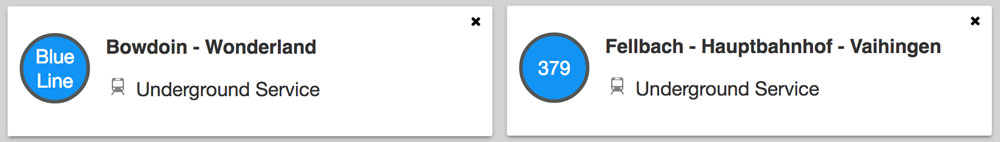
\includegraphics[width=\textwidth]{gtfs_differences.jpg}
        \caption{UI Element mit GTFS Informationen}
        \label{fig:gtfs_differences}
      \end{center}
    \end{figure}

    Links in der Abbildung ist die Korrekte Bezeichnung der Route zu sehen nämlich \texttt{Blue Line}, wohingegen rechts nur eine numerische ID zu sehen ist, die nicht für den Nutzer vorgesehen und damit falsch ist. Damit die rechte Seite korrekt wäre müsste dort \texttt{U1} abgebildet sein. Die fehlende beziehungsweise nicht gegebene Übereinstimmung der beiden Feeds führt also zu Problemen bei der Darstellung die auch durch die Verwendung eines anderen Feldes wie zum Beispiel \texttt{route\_short\_name} nicht behoben werden können.\\

    Um sich den Inhalt einer GTFS-Datei besser vorstellen zu können ist nachfolgend ist ein Auszug der \texttt{stops.txt} Tabelle abgebildet.

    \begin{lstlisting}[captionpos=b, caption=Auszug der ersten Zeilen von \texttt{stops.txt}, label=lst:gtfs-auszug]
      stop_id,stop_name,stop_lat,stop_lon
      668,Moetzingen Bruehlstrasse,48.53249,8.775416
      2840,Ludwigsburg Mainzer Allee,48.9018,9.21601
      6409,Burgholzhof,48.81742,9.191285
      6824,Neuenhaus Groerach,48.62443,9.213599
      152,Jux,49.030426,9.438538
    \end{lstlisting}

		Da das GTFS-Format das grundlegende Datenformat für diese Arbeit ist, sollen nachfolgend kurz die wichtigsten Tabellen beschrieben werden.

		\begin{itemize}
			\item \texttt{agency.txt}: Beinhaltet Informationen über die Verkehrsunternehmen, welche das Feed und die Daten bereitstellen.

			\item \texttt{routes.txt}: Eine Route ist eine Gruppierung von Trips. Die verschiedenen Eigenschaften einer Route werden in dieser Tabelle gespeichert.

			\item \texttt{trips.txt}: Ein Trip gehört zu einer Route. Eine Route kann dabei beliebig viele Trips haben. Welche Trips aktiv sind wird durch den Kalender festgelegt.

			\item \texttt{calendar.txt}: Bestimmt, an welchen Tagen ein Trip aktiv ist.

			\item \texttt{stop\_times.txt}: Diese Tabelle beschreibt welche Stationen nacheinander angefahren werden. Für jede Station beinhaltet sie die Ankunfts- und Abfahrtszeiten.

			\item \texttt{stops.txt}: Stellt nähere Informationen für jede Station zur Verfügung wie zum Beispiel den Stationsnamen und deren Position.

			\item \texttt{shapes.txt}: Jeder Trip kann eine dazugehörigen Polyline\footnote{Linienverlauf} haben. Eine Polyline ist dabei nichts anderes als eine Abfolge von Punkten, die, wenn man sie verbindet, eine Linie ergeben. Um einen Routenverlauf auf eine Karte zu zeichnen, wird diese Tabelle folglich unbedingt benötigt. 
		\end{itemize}

  Ein UML-Diagramm, welches die in relation stehenden Datien aufzeigt, existiert unter folgender Adresse: \url{https://developers.google.com/transit/gtfs/reference/} 

\end{newpage}
% section grundlagen